% !TeX spellcheck = it_IT
%Slide 4 per l'indice, come strutturarlo?
%Using Slide set 1
\section{Principi di Teoria della Trasmissione}

%Maybe? Idk if it's significant
%	\subsection{Introduzione}
%	
%	Con i diversi tipi di rete abbiamo diversi \textbf{range} d'operazione: 
%	\begin{itemize}
	%		\item \textbf{Bluetooth} e \textbf{PAN} (Personal Area Network): estremamente corto raggio, range dell'ordine dei metri
	%		\item \textbf{Wifi}: Relativamente corto raggio, ma nomadico, ti puoi muovere, anche se non troppo, di solito all'intero di un'area definita
	%		\item \textbf{LTE, 5G}: nomadico davvero, ti puoi muovere come vuoi
	%	\end{itemize}
%	
%	Ciascuna di queste tecnologie ha delle particolarità ed è pensata per supportare un determinato tipo di servizi/casi d'uso. Con il progredire del tempo le soluzioni diventano sempre più specifiche rispetto alla situazione per cui sono pensate. Verrà trattata un po' l'evoluzione delle reti. Dal 5G in poi in particolare, anche il lato software è modificabile e permette più innovazione. \\
%	
%	\textbf{Edge computing}: stesse caratteristiche del cloud computing (risorse virtualizzate on demand), ma le vuole fornire a più basso livello. Fog computing (cloud sta in alto, nebbia in basso, ovviamente). Una delle tecnologie abilitanti del 5g.\\
%	
%	Guida assistita e autonoma: ha requisiti stringenti, real time, scenario imprevedibile, cooperative perception, scenario eterogeneo e complesso.
%	
%	Smart Factories: industria 4.0, all'interno di una fabbrica bisogna gestire tutta la parte robotica in un closed loop: sensing, fusione e contesto, decisione, attuatori. Tutto questo loop necessita di real time, sicurezza e coordinamento. 

Vogliamo \textbf{trasmettere informazioni} binarie su un \textbf{mezzo analogico}. Tipicamente abbiamo uno schema del tipo: 
\begin{center}
	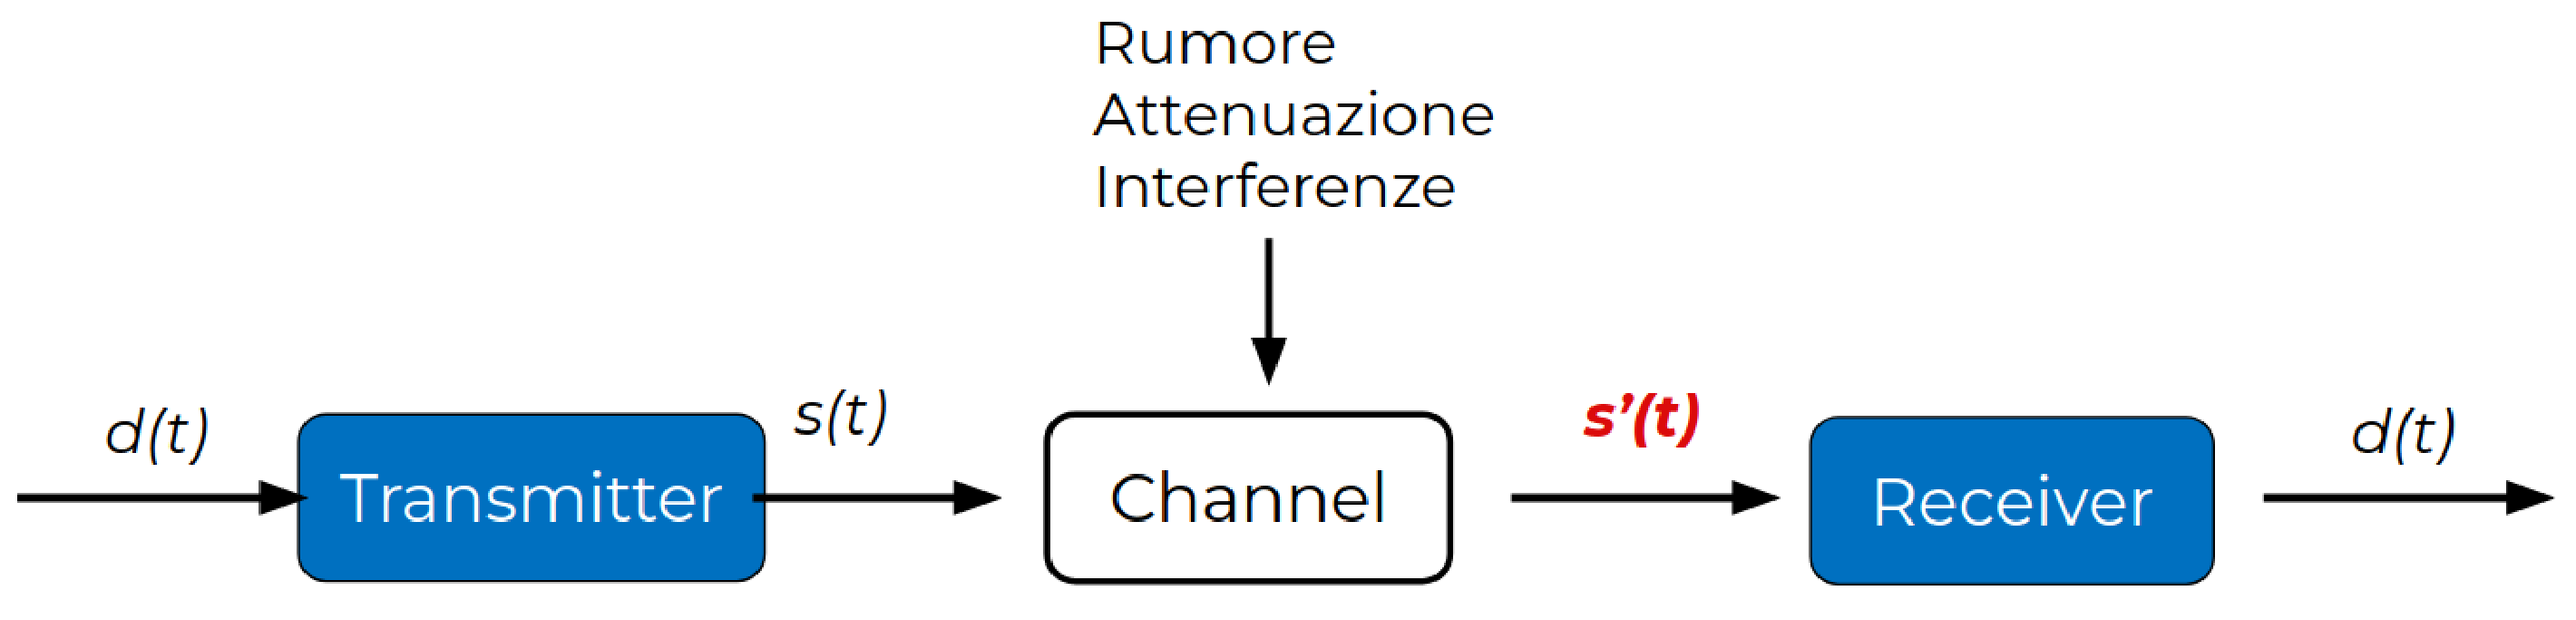
\includegraphics[width=0.95\linewidth]{img/PTT/tr-scheme}
\end{center}
Si hanno dati nel tempo i quali passano da un \textbf{trasmettitore} il quale "traduce" i dati \textbf{digitali} in un segnale \textbf{analogico}, il quale può essere \textbf{trasmesso su un mezzo analogico} (e.g., aria, cavi, ecc.). Il segnale attraversa il mezzo e arriva a un ricevitore, il quale decodifica il segnale per tornare ai dati originali. Però, il canale non è perfetto o perfettamente affidabile, è possibile \textbf{introduca}:
\begin{itemize}
	\item Il \textbf{rumore} in mezzi wireless può essere importante
	\item Il ricevitore deve essere in grado di recepire piccole quantità di potenza, in quanto il segnale potrebbe essere \textbf{attenuato}
	\item \textbf{Interferenze}, "casuali" dovute alla stessa tecnologia (propagazione del mezzo, ecc.) oppure volontarie (e.g., jamming).
\end{itemize}
Quindi il \textbf{segnale inviato} risulterà \textbf{diverso} dal \textbf{segnale ricevuto}, ma se il segnale viene strutturato correttamente ed è robusto a queste deformazioni il ricevitore sarà in grado di estrapolare ugualmente dati dal segnale "modificato". Quanto è facile ricostruire il segnale dipende da \textbf{quanto} i fenomeni di disturbo hanno \textbf{modificato} il segnale, può pure non essere ricostruibile. \\

Per \textbf{segnale}
\begin{itemize}
	\item \textbf{analogico:} si intende una variazione continua, senza interruzioni o discontinuità
	\item \textbf{digitale:} un livello di segnale viene mantenuto costante per un determinato intervallo, con un cambio di livello rapido (quasi istantaneo)
\end{itemize}

Vogliamo passare da una forma d'onda all'altra (trasmettitore e ricevitore fanno questo). \\

\newpage

\subsection{Rappresentazione dei segnali}

\paragraph{Dominio del tempo:} Un segnale può essere visto nel dominio del tempo come un \textbf{segnale periodico sinusoidale}
$$ s(t) = A \sin (2 \pi ft + \phi) $$

Dove: 
\begin{itemize}
	\item \textbf{Ampiezza} $(A)$:	massimo livello o forza del segnale nel tempo (Volt)
	\item \textbf{Frequenza} $(f)$: Numero di cicli al secondo (Hz)
	\item \textbf{Fase} $(\phi)$: posizione relativa all'interno del periodo
	\item \textbf{Periodo} $(T)$: tempo impiegato per un ciclo ($1/f$)
	\item \textbf{Lunghezza d'onda} ($\lambda$): distanza occupata da un singolo ciclo: $\lambda = c/f$ oppure $\lambda = T c$ dove $c = 3\cdot 10^8$ m/s
\end{itemize}
La variazione di ampiezza, fase e frequenza vengono usate per codificare le informazioni (e.g., radio AM e FM, modulazione di fase non per le radio, ma alter cose).

\paragraph{Dominio delle frequenze:} Possiamo considerare un'onda elettromagnetica guardandola nel tempo, ma anche nel dominio delle frequenze. \textbf{Ogni segnale} (ragionevolmente periodico) \textbf{può essere scomposto da una serie di segnali periodici} (onde seno e coseno) con ampiezza, frequenza e fase differenti: trasformata di Fourier
$$ s(t) = \frac{1}{2} c + \sum_{n=1}^{\infty} a_n \cdot \sin (2 \pi n f t) + \sum_{n=1}^{\infty} b_n \cdot \cos (2 \pi n f t) $$
Dove: 
\begin{itemize}
	\item $f=1/T$: frequenza \textbf{fondamentale} $(n=1)$
	\item $a_n, b_n$: \textbf{ampiezza} delle \textbf{singole componenti}, dette armoniche
	\item $c$: costante che rappresenta il \textbf{valore medio} del \textbf{segnale}
\end{itemize}
Possiamo \textbf{scomporre} un segnale in \textbf{diverse armoniche}, ognuna con il suo "contributo" rispetto al segnale originale. Questa è la serie di Fourier discreta, in un calcolatore saranno un numero finito di frequenze e la versione originale era con gli integrali, nel continuo.\\

\newpage

Insomma, serve per passare da un dominio all'altro.

\paragraph{Cosa ci interessa:} Dal punto di vista di un ricevitore, il quale riceverà tali segnali, ci interessa capire \textbf{com'è composta l'onda} a partire \textbf{da un'osservazione nel tempo} di quest'onda. Come faccio a \textbf{risalire alle componenti} a partire da un'osservazione nel tempo della forma d'onda? Le domande sono: 
\begin{enumerate}
	\item Come si fa a \textbf{determinare} le \textbf{ampiezze} di ciascuna componente
	\item Con quale \textbf{frequenza campionare il segnale}? Il mondo digitale è discreto per definizione, in che punti della curva bisogna "leggere" per poter ricostruire l'onda in maniera precisa
\end{enumerate}

\paragraph{Teorema del campionamento di Shannon:} La \textbf{frequenza di campionamento} deve essere almeno il \textbf{doppio della frequenza massima del segnale} in ingresso. \\
Sapendo la frequenza massima (e tra ricevitore e trasmettitore ci si mette d'accordo), devo campionare ad almeno il doppio per evitare perdita di dati. \\

\paragraph{Passaggi di dominio:} Per passare da un dominio all'altro abbiamo due algoritmi:
\begin{itemize}
	\item \textbf{Fast Fourier Transform FFT:} da tempo a frequenze, passandogli la forma d'onda nel tempo restituisce le componenti
	\item \textbf{Inverse Fast Fourier Transform IFFT:} da frequenze a tempo, partendo dalle componenti restituisce la forma d'onda
\end{itemize}

Con "componenti" si intende i coefficienti $a_n$ e $b_n$ viste nella serie di Fourier. Questi algoritmi sono semplici, vengono implementati tramite hardware nei dispositivi, i quali devono effettuarle costantemente. \\

Assegnando dei bit al fingerprint di una forma d'onda (valori della trasformata), posso creare una lookup table per trovare il "significato" di una forma d'onda a partire dalla sua trasformata (osservo l'onda, faccio la trasformata, lookup per il significato).\\

\newpage

Nel dominio delle frequenze: quando \textbf{tutte le frequenze} sono \textbf{multipli interi di una frequenza base}:
\begin{itemize}
	\item $f=$ \textbf{frequenza fondamentale}
	\item $kf =$ \textbf{armonica} ($k>1$)
\end{itemize} 

\paragraph{Periodo:} Il periodo di $s(t)$ è il periodo della frequenza fondamentale $(T = 1/f)$.

\paragraph{Spettro:} Lo spettro del segnale è il range di frequenze che lo contiene (da dove a dove vanno le frequenza).

\paragraph{Banda:} Absolute bandwidth è l'ampiezza dello spettro ("larghezza" dello spettro). \\

\newpage

\subsection{Relazione tra Bandwidth e Data Rate}

Esempio: vogliamo trasmettere un'onda quadra come \textbf{composizione finita di onde sinusoidali}. Esempio:
\begin{center}
	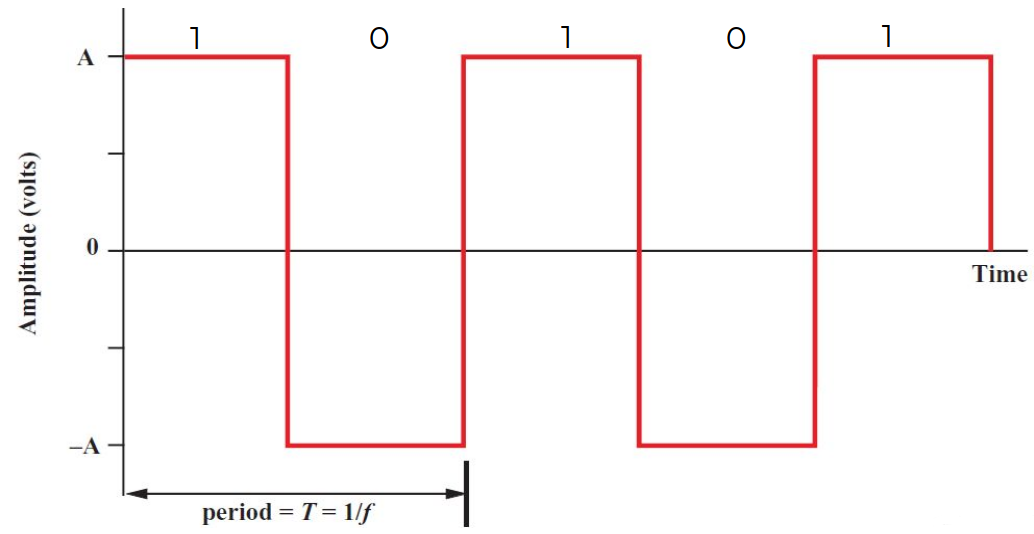
\includegraphics[width=0.7\linewidth]{img/PTT/quadra1}
\end{center}

Trasmettiamo 2 bit per ogni periodo, ovvero un data rate di 2 bit. Possiamo avere una \textbf{sommatoria} infinita di onde \textbf{sinusoidali}: 
$$ s(t) = A \cdot \frac{4}{\pi} \cdot \sum_{k \text{ odd}, k=1}^{\infty} \frac{\sin (2 \pi kft)}{k} $$
Ma questo richiederebbe una banda infinita, il che è difficile, quindi possiamo \textbf{ridurre lo spettro} per ottenere un'\textbf{approssimazione}: 
\begin{center}
	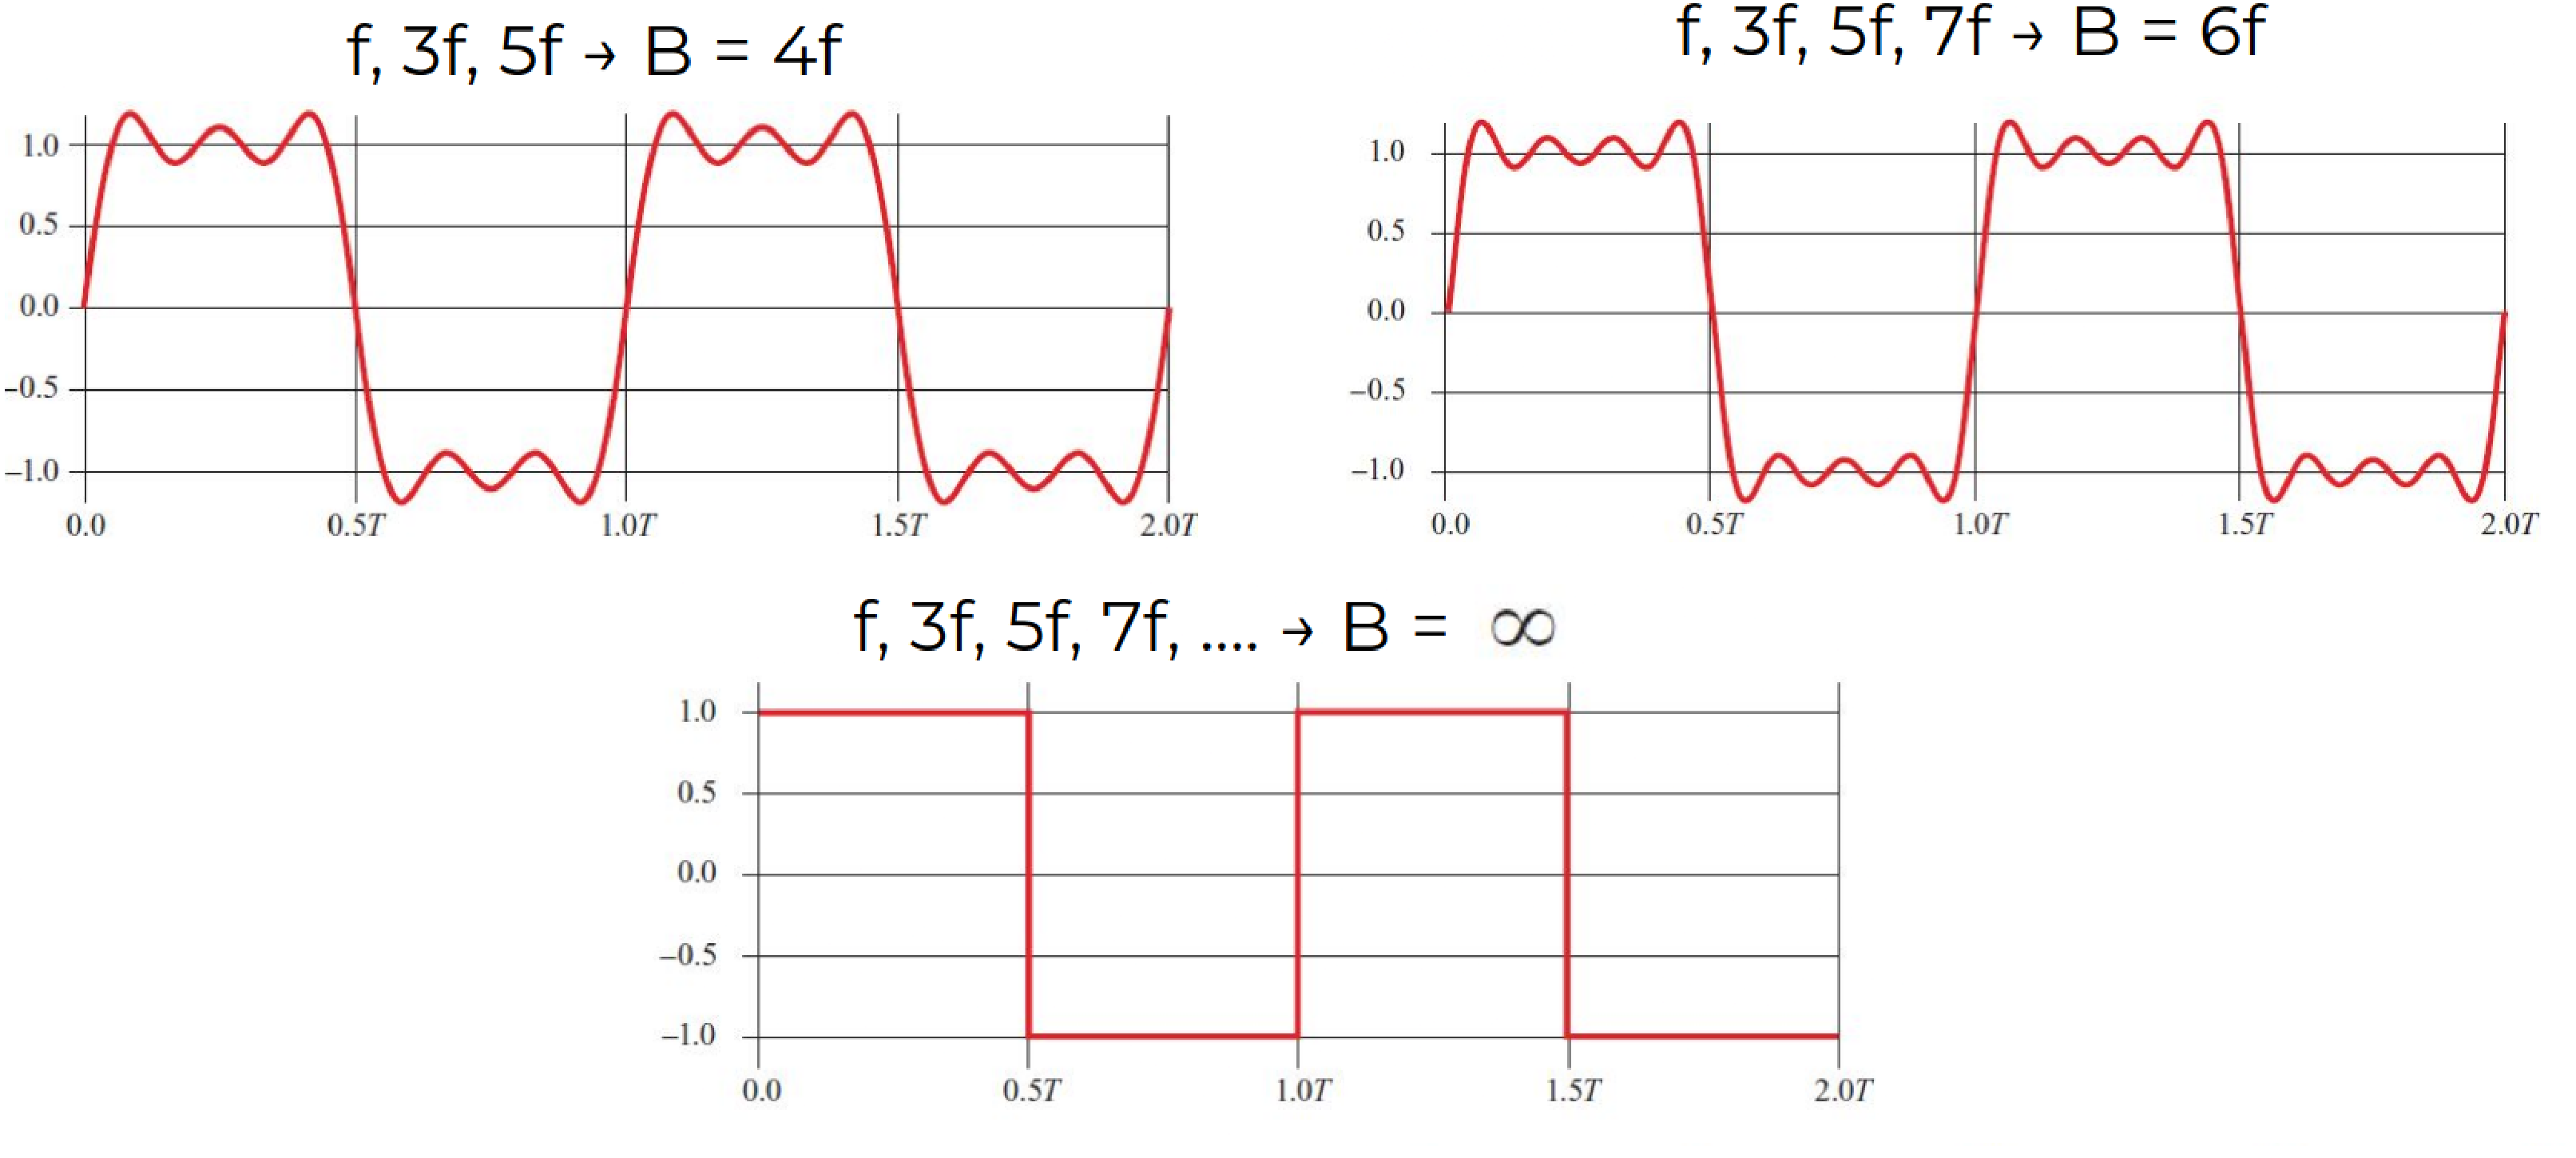
\includegraphics[width=\linewidth]{img/PTT/fourier1m}
\end{center}

Nel primo esempio una banda di $4f$ che va da $f$ a $5f$, nel secondo aumentiamo la banda a $6f$, migliorando l'approssimazione.
Con la banda che tende all'infinito otteniamo l'onda originale.

\newpage

Con una certa banda, \textbf{quanti dati possiamo trasmettere?} Esempio: 
\begin{center}
	\begin{tabular}{| c | c | c |}
		\hline
		Freq. fondamentale $(f)$ & 1 MHz & 2 MHz \\
		\hline
		Spettro & 1 Mhz - 5 Mhz & 2 Mhz - 10 Mhz \\
		\hline
		Periodo (T) & 1 $\mu$s & 0.5 $\mu$s \\
		\hline 
		Durata di 1 bit & 0.5 $\mu$s & 0.25 $\mu$s \\
		\hline
		Bandwidth (B) & 4 Mhz ($5f - f$) & 8 Mhz ($2(5f - f)$) \\
		\hline
		Data rate (bps) & 2 Mbps (2 bit/$\mu$s) & 4 Mbps (4 bit/$\mu$s) \\ 
		\hline
	\end{tabular}
\end{center}
Con il doppio della banda abbiamo raddoppiato il data rate.\\

\paragraph{Capacità del canale:} Quanti bit possiamo trasmettere sul canale senza perdere informazioni?
\begin{itemize}
	\item \textbf{Channel capacity:} massimo bit rate alla quale è possibile trasmettere dati su un canale di comunicazione in determinate condizioni
	\item \textbf{Noise:} segnale NON voluto che si combina al segnale trasmesso, distorcendolo
	\item \textbf{Error rate:} tasso di errore (bit error rate), quante volte viene modificato involontariamente il segnale
\end{itemize}

Come possiamo trasmettere la \textbf{stessa quantità di informazioni senza usare più banda}? La soluzione è \textbf{ridurre il numero di armoniche}, semplificando la forma d'onda e peggiorando l'approssimazione. Questo si può fare finché l'onda non è un'approssimazione "troppo approssimata" (deve essere distinguibile).\\

\paragraph{Considerazioni:} Vogliamo trasmettere una banda infinita con banda finita, ma una banda minore porta a distorsione maggiore. Una soluzione potrebbe essere scegliere la banda finita più ampia; sarebbe fattibile ma ci sono costi economici (i.e., la banda non è gratis) e il dispositivo deve essere in grado di gestirla. Inoltre può creare rumore aggiuntivo. \\

\paragraph{Nyquist Bandwidth:} Dato un canale noise-free (ideale) la bandwidth limita il data-rate. Il \textbf{limite della quantità di informazioni} (misurata in bit/secondo e multipli) è limitato da due volte la banda
$$ C = 2B $$
per \textbf{segnali binari} (2 livelli di voltaggio). Per \textbf{segnali multilivello}, codificare i dati su più livelli di segnale
$$ C = 2B \log_2 M $$
Dove $M$ è il numero di livelli.\\

La \textbf{capacità del canale aumenta con il numero di possibili livelli} in cui codificare il segnale, modificando uno dei parametri (ampiezza, frequenza, fase). Il numero di livelli di segnale aumenta il numero di bit che si possono trasmettere con ogni trasmissione: con 2 valori trasmettiamo 1 bit, con 8 possibili valori possiamo trasmettere 3 bit alla volta. \\

Questo possibile solo se non c'è rumore, il massimo possibile. Tenendo il considerazione il rumore la capacità si abbassa.

Esempio di effetto del rumore sul segnale trasmesso: 
\begin{center}
	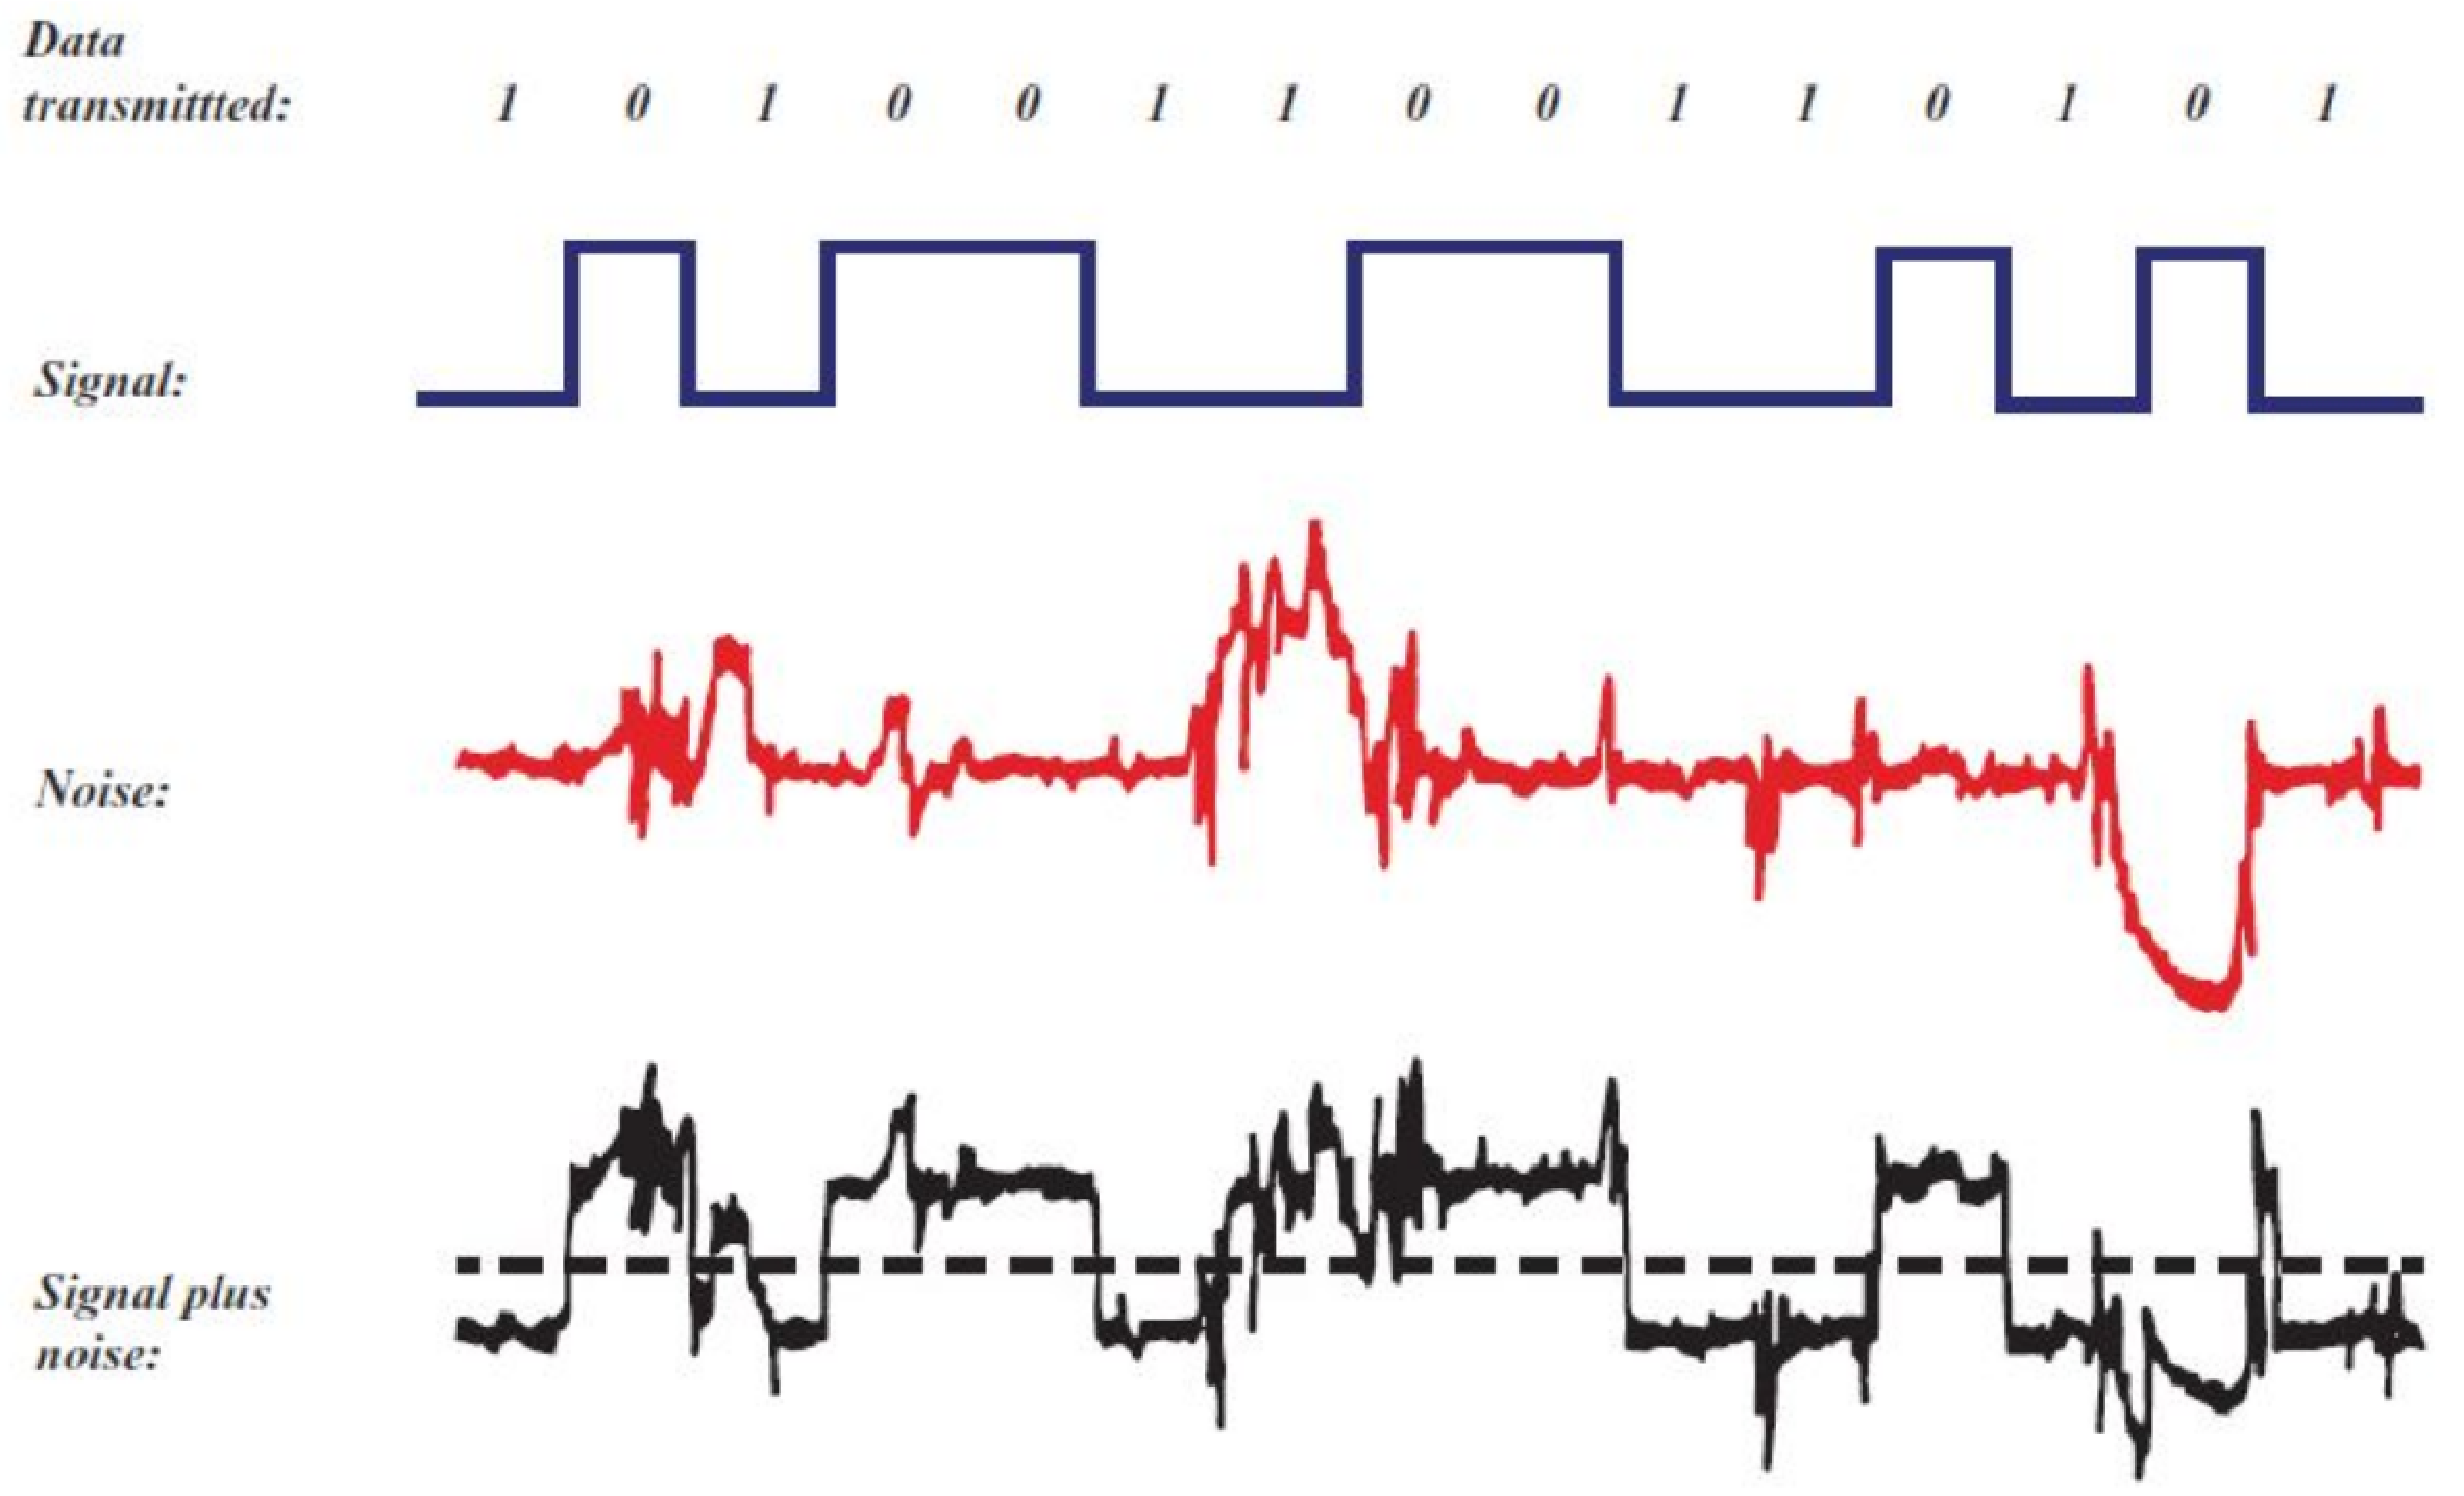
\includegraphics[width=\linewidth]{img/PTT/errors1}
\end{center}
Considerando il profilo temporaneo del rumore, il ricevitore riceve un segnale diverso, con modifiche su cui non abbiamo controllo, indipendenti da ricevitore e trasmettitore.\\

% End L1